\documentclass{article}

\usepackage{neurips_2025_ml4ps}

\usepackage[utf8]{inputenc}
\usepackage[T1]{fontenc}
\usepackage{amsmath,amssymb,amsthm}
\usepackage{booktabs}
\usepackage{graphicx}
\usepackage{microtype}
\usepackage{bm}
\usepackage[hidelinks]{hyperref}
\usepackage{url}

% Venue-neutral build: the style file's workshop notice box is suppressed so that
% no venue string appears in the artifact.
\makeatletter
\renewcommand{\@notice}{}
\makeatother

\title{The Price of a Flat Direction:\\ Transverse Curvature Sets Retention in a Trained Recurrent Memory}

\author{}

\begin{document}
\maketitle
\begin{abstract}
Recurrent neural networks are capable of storing continuous latent values on a manifold of marginally stable states. Prior work establishes that such a manifold is fundamentally fragile: noise diffuses the state along the manifold, most infinitesimal perturbations to the dynamics destroy it, and exact equivariance protects a neutral direction with zero Lyapunov exponents tangent to the group orbit. \emph{However}, while the kinematics of symmetry protection are known, the quantitative exchange rate---how the retention of a written value scales with the transverse curvature of a trained potential---remains unmeasured. \emph{In this work, we measure this constitutive exchange rate} on a trained potential. We evaluate a recurrent unit that advances a latent state $(q,p)$ via a damped symplectic velocity-Verlet step of a learned Hamiltonian. The trained potential $V_\theta$ is $G$-invariant with minimisers on a $G$-orbit, representing spontaneous symmetry breaking, such that the curvature $\mu$ transverse to the orbit determines the survival time of a written value. We measure this retention profile at latent dimension $4$ on an $S^1$ testbed, across $\le5$ seeds on a laptop CPU. The retention half-life follows $n_{1/2}\propto\mu^{-2}$, with a fitted overdamped slope of $-0.985$ (against a predicted $-1$), and the underlying curvature identity holds exact to $1.000000\pm5\!\times\!10^{-12}$ over $4.5$ decades. This scaling law halts at a crossover boundary $\varepsilon\mu\approx\gamma/2$, beyond which the half-life saturates at a curvature-independent floor. Furthermore, this retention profile survives the training-time correction required to maintain the orbit, holding at $\approx20\times$ the temporal horizon where the objective naturally degrades it. To validate these findings on a learned system, we apply a recent single-exponential lifetime estimator unchanged on our trained checkpoints. The estimator matches our overdamped predictions to $\le3\%$ below the crossover but mispredicts by $\approx3.2\times$ above it in the calculable direction. Finally, we explicitly bound these results by identifying where the laws do not extend: symmetric training data alone fails to produce a near-flat direction on this architecture class (a gap of $13$--$14$ orders in $\mu^2$); the continuous coset register is strictly designed; and the retention advantage against recurrent baselines inverts under compute normalization. All designed-testbed results serve as verification of the theory, while learned-system results provide empirical evidence.
\end{abstract}

\section{Introduction}\label{sec:intro}

A recurrent state designed to hold an analog value relies on a flat direction: a continuous set of states that the network dynamics do not distinguish, ensuring a written value neither decays nor converges to a preferred attractor. Symmetries supply these directions natively through spontaneous symmetry breaking. If a learned potential $V_\theta$ is $G$-invariant but its minimiser is not, the minimisers form a $G$-orbit where the Hessian annihilates every orbit tangent, leaving the orbit coordinate neutral. This neutral coordinate acts as the Nambu--Goldstone mode of the trained potential and functions as the continuous register. \emph{However}, while the theoretical existence of such a flat direction is established, its operational utility depends on a quantitative price list: how much retention is gained for a given transverse curvature, the boundaries of this scaling law, and the stability of the manifold against corrective training mechanisms. \emph{Therefore, we explicitly measure these three properties on trained models.}

We analyze an architecture that advances a phase-space state $(q,p)$ through a symplectic velocity-Verlet step using a learnable separable Hamiltonian $H(q,p)=T(p)+V_\theta(q)$. A per-step damping map $p\mapsto(1-\gamma)p$ is applied to supply controllable forgetting. This work does not propose a new architecture, but rather provides a closed-form analysis of retention on a trained symplectic recurrent model. The reference unit evaluated is the Causal Learning Unit (CLU), introduced as CHLU in Jawahar \& Pierini (2026). Our results hold generally for the class of damped symplectic recurrences, guided by an exactly-solvable underlying theory (developed in the supplementary Anonymous, 2026, hereafter \emph{the theory note}).

\paragraph{Definitions and conversions.} To understand the motivation for this work better, we start with a short primer on the two distinct ``mass'' quantities utilized, which operate in inverse alignment.
\begin{itemize}
    \item \textbf{Inertial mass ($M_i$):} The learned diagonal entries of the kinetic term $T$. A larger $M_i$ yields slower dynamics.
    \item \textbf{Spectral mass ($\mu_k$):} Defined here as the \emph{transverse curvature}, where $\mu_k^2=\lambda_k(M^{-1/2}\nabla^2V_\theta M^{-1/2})$ at a critical point. A larger $\mu$ results in shorter memory retention.
\end{itemize}
All retention laws in this paper are formulated using $\mu$. Crucially, we avoid arbitrary unit rescaling between inverse time (flow-Jacobian eigenvalues or Lyapunov exponents) and inverse time squared ($\mu^2$, eigenvalues of a mass-whitened potential Hessian). Instead, cross-field comparisons (Sec.~\ref{sec:headtohead}) are performed strictly by running published rate-based estimators unchanged on our trained models. Furthermore, what the broader literature refers to as \emph{memory lifetime} is standardized here as the half-life $n_{1/2}$, measured in map applications. Metrics such as time constants ($\tau$) or diffusion coefficients ($D$) are evaluated and reported explicitly alongside the condition that defines them, as these metrics bifurcate past critical crossover thresholds.

\paragraph{Contributions.} This paper provides a summary of the transverse-curvature price list of a trained recurrent memory. We structure our contributions as follows:
\begin{enumerate}
\item \emph{The price list} (Sec.~\ref{sec:pricelist}, Sec.~\ref{sec:cure}): We establish the relationship between transverse curvature and retention, identify the crossover boundary where this law halts, and demonstrate the survival of this relationship under training-time corrections that preserve the orbit.
\item \emph{Evidence on a learned system} (Sec.~\ref{sec:headtohead}): We evaluate a recently posted single-exponential lifetime estimator directly on our trained checkpoints. It aligns with our price list in the overdamped regime but predictably fails above the crossover boundary.
\item \emph{Operational boundaries and negative results} (Sec.~\ref{sec:boundary}): We explicitly outline the limits of our findings. On this architecture class, flat directions must be designed rather than trained for; the continuous register does not transfer to an emergent potential; and the retention efficiency relative to recurrent baselines inverts when normalized for compute.
\end{enumerate}
Results derived from designed testbeds (e.g., invariant potentials, analytic tilts, spurions) serve as verification of the exact theory. Conversely, outcomes from learned-system, training-dynamics, and comparative baseline experiments are presented as empirical evidence.

\section{Related work}\label{sec:related}

The intersection of temporal deep learning dynamics and symmetry-driven learning frameworks converges on the continuous attractor. Neutrality along group-orbit directions is a foundational principle (Golubitsky, Stewart \& Schaeffer 1988; Krupa 1990; Rumberger 2001). This structure operates as a continuous attractor: a manifold where tangent directions are marginally stable and normal directions are strictly stable (S\'agodi et al.\ 2024). It serves as the theoretical substrate for neural integrators (Seung 1996) and measurable toroidal codes in biological systems (Kim et al.\ 2017; Gardner et al.\ 2022; Khona \& Fiete 2022). We clarify that our work models artificial computational constraints and makes no claims regarding biological data.

The literature establishes fundamental constraints on continuous attractors. Noise drives diffusion along the manifold, lower-bounded by the code's Fisher information (Burak \& Fiete 2012). Furthermore, these manifolds are structurally unstable and generally destroyed by infinitesimal perturbations to the dynamical rules, an issue termed the \emph{fine-tuning problem} in online learning (S\'agodi et al.\ 2024). Homeostatic mechanisms to restore these flat directions are well-documented (Renart, Song \& Wang 2003), and local learning rules have been shown to produce accurate ring-attractor tuning (Vafidis et al.\ 2022). Approximate continuous attractors also emerge analytically during task training (Dinc et al.\ 2025). \emph{However}, the literature currently lacks a precise exchange rate on trained models linking transverse curvature to retention capacity, including the crossover bounds of such laws. \emph{We address this gap} by quantifying this relationship in closed form, outlining regime transitions (floors and crossovers) that cannot manifest in first-order dynamical systems.

\paragraph{Delineation from current literature.} Recent work on \emph{flow equivariance} (Keller 2025) extends one-parameter Lie-group symmetries through time within recurrent states to maintain long-horizon coherence in world models (Lillemark et al.\ 2026). We explicitly note that ``flow'' refers to a one-parameter Lie subgroup acting through time, rather than Ricci or normalizing flows. While we study the same object---continuous symmetry in a recurrent state---our focus differs. Flow-equivariant models target velocity extrapolation; we isolate and price the retention cost of transverse curvature without making generalization claims. Similarly, concurrent workshop work has explored soft symmetry regularization for continuous attractors. In contrast, our designed framework builds the symmetry by construction, while our emergent models utilize no symmetry regularizers, informing our boundaries in Sec.~\ref{sec:boundary}. Finally, regarding training dynamics, literature shows that temporal-consistency regularizers shape attractor geometry (Haputhanthri et al.\ 2025). We analyze the inverse dynamic in Sec.~\ref{sec:cure}: our primary objective erodes a designed flat direction, necessitating an anchor to preserve it.

\paragraph{Protection mechanisms and Lyapunov spectra.} A recent preprint (arXiv:2605.03338) theoretically proves that a $C^1$ field exactly equivariant under a Lie group guarantees at least $\dim(G/\mathcal H)$ zero Lyapunov exponents tangent to the orbit. It further demonstrates that controlled symmetry breaking yields a finite memory lifetime on an $S^1$ path integration task. We do not claim novelty over these qualitative lifetime predictions or existence proofs. Instead, we contribute the exact exchange rate mapped onto a trained potential. The currencies are fundamentally distinct: Lyapunov exponents provide inverse time (kinematics), whereas our $\mu^2$ provides the transverse curvature of a potential, scaling as inverse time squared (constitutive dynamics). Lyapunov spectra evaluate vector transport but do not capture the specific latching or noise accumulation mechanics required for functional memory. We explicitly adopt the breaking-and-censoring protocol from arXiv:2605.03338 in Sec.~\ref{sec:headtohead} to run their estimator unchanged on our models.

Prior work by Xu et al.\ (2023) maps Lie-group representations into recurrent grid-cell networks, enforcing a torus topology over a continuous attractor. We share this geometry but introduce a precise price list for temporal retention. Related studies optimize attractor state packing (Vastola 2024) and approach memory modification through geometry (D\"onmez 2024). Furthermore, our designed-versus-emergent analysis mirrors the exact-equivariance-versus-symmetry-breaking dichotomy (van der Ouderaa \& van der Wilk 2023; Iqbal et al.\ 2026). Utilizing level sets to analyze tuning landscapes is established (Akhtiamov \& Thomson 2023; Wang \& Ponce 2023), as is leveraging canonical quotient coordinates (Aslan, Platt \& Sheard 2023) and engineering equivariant memories (Di Bernardo et al.\ 2025). We separate our work from cross-session representational drift (Driscoll et al.\ 2017; Aitken et al.\ 2022; Jude et al.\ 2023), focusing entirely on coset coordinate motion governed by our explicit dynamics. Standard baselines include LSTM (Hochreiter \& Schmidhuber 1997), LEM (Rusch et al.\ 2022), and coRNN (Rusch \& Mishra 2021a), supported by conformal symplecticity principles (McLachlan \& Perlmutter 2001) and wake--sleep contrastive divergence (Hinton et al.\ 1995; Tieleman 2008), which classically distorts energy landscapes (Fischer \& Igel 2010; Nijkamp et al.\ 2020).

\paragraph{Positioning boundaries.} To clearly scope our contribution, we explicitly retire four claims (detailed fully in Appendix~\ref{app:pos}). \emph{(1)} Attention and state-space models possess retention-guarantee analogues (e.g., HiPPO-LegS, Gu et al.\ 2020). \emph{(2)} Framing retrieval as a rollout rather than a weighted sum is established by Kong, Brewer \& Lai (2024). \emph{(3)} Continuous dynamics do not bypass the soft-memory lineage of NTMs and DNCs (Graves et al.\ 2014, 2016; Csord\'as \& Schmidhuber 2019). \emph{(4)} This framework is not positioned as a competitor to transformer architectures. Our specific contribution remains a physics-structured associative memory where retention is governed as a designed, per-item property controlled by $\mu^2$. The closest parallel architecture is Titans (Behrouz et al.\ 2025), which utilizes discretized damped second-order dynamics for associative memory. We differ by reading out and pricing the damping and inertia natively, rather than treating them as optimizer hyperparameters.

\section{Setup}\label{sec:setup}

\paragraph{Dynamical mapping and retention bands.} We lay the foundations for the discrete map. One dissipative velocity-Verlet step (defined by step $\varepsilon$ and damping $\gamma$) advances $(q,p)$ via a kick--drift--kick of the Hamiltonian $H=T(p)+V_\theta(q)$, followed by the damping map $p\mapsto(1-\gamma)p$. This map is conformally symplectic, satisfying $J^\top\Omega J=(1-\gamma)\Omega$ and $\det J=(1-\gamma)^d$. Phase-space volume subsequently contracts by a fixed factor at each step, preserving geometry while diminishing scale. The memory dynamics at each normal mode reduce to a $2\times2$ block defined by $\mu^2=k/m$ and $h=\varepsilon\mu$. The retention behavior splits into three explicit bands:
\begin{itemize}
    \item \textbf{The Latch:} ($\mu=0$, symmetry-protected). Exhibits frozen displacement $q_\infty=q_0+\varepsilon p_0/(M\gamma)$ and an infinite half-life.
    \item \textbf{The Overdamped Register:} ($0<\varepsilon\mu\lesssim\gamma/2$). Resolves to a half-life of $n_{1/2}\approx2\gamma\ln2/[(2-\gamma)(\varepsilon\mu)^2]$.
    \item \textbf{The Underdamped Working Memory:} ($\gamma/2\lesssim\varepsilon\mu<2$). Bound by a curvature-independent envelope half-life of $2\ln2/(-\ln(1-\gamma))$.
\end{itemize}
The boundary separating the overdamped and underdamped regimes is the exceptional point $h^*\approx\gamma/2$, where the block matrix becomes defective. In this map, relaxation onto the orbit dictates the fast normal flow, while retention governs the slow tangent flow. Unlike standard neural integrators that store values by removing damping, our flat mode requires $\gamma>0$ to prevent infinite drift, effectively forming an exact latch.

\paragraph{Curvature instantiation and coset storage.} We constrain this framework to critical points of $V_\theta$, where the transverse curvature realizes one of three states on our trained models. \emph{First}, $\mu^2$ is exactly zero along $\dim(G/\mathcal H)$ directions when the trained minimisers form a $G$-orbit, indicating spontaneous symmetry breaking (the designed Nambu--Goldstone mode). \emph{Second}, $\mu^2$ is small but positive when an explicit algorithmic tilt breaks the orbit, creating a pseudo-Goldstone slow manifold (instantiated via analytic tilts in Appendix~\ref{app:gmor} and generic MLPs). \emph{Third}, $\mu^2$ is strictly positive when the minimiser is invariant, eliminating the orbit entirely (observed in the eroded vacuum of Sec.~\ref{sec:cure}). We rely strictly on the classical, tree-level Goldstone theorem evaluated over a Hessian. The architecture stores the \emph{coset coordinate}---the position along the flat direction. The parameters $(\varepsilon,\gamma,T)$ map specific $\mu^2$ values to exact retention lifetimes via the three bands.

\paragraph{Operational Assumptions and Scopes.} All models evaluated utilize the Experiment-D configuration of the reference unit: dimension $4$, hidden size $64$, learned-Newtonian kinetic term, $\mathrm{dt}=0.05$, a unit circle at $256$ points, and $150$ epochs (justification for avoiding $1000$ epochs is provided in Sec.~\ref{sec:cure}). Checkpoints belong to either the \emph{designed} family (an architecturally-$SO(2)$-invariant $V_\theta$ on $5$ seeds) or the \emph{emergent} family (a generic MLP $V_\theta$ on $3$ seeds).
\begin{itemize}
    \item \textbf{Finite Temperature Latches:} The infinite half-life of the latch is a deterministic, $T=0$ property. At $T>0$, the coset diffuses with coefficient $D_\theta=\varepsilon T(2-\gamma)/(2F^2\gamma)$, yielding a finite computable lifetime (verified on designed checkpoints where increasing friction from $\gamma=0.05$ to $0.2$ lengthens memory by $3.77\pm0.23\times$). All Sec.~\ref{sec:results} measurements are conducted at $T=0$.
    \item \textbf{Kinetic Breaking:} A flat direction maintains $\mu^2=0$ under inertial anisotropy by Sylvester's law of inertia. Map equivariance protects the current, but flatness protects the register.
    \item \textbf{Tilt Limitations:} The \emph{tilt-as-a-dial} construction is exclusively verified on designed geometries. As detailed in Appendix~\ref{app:neg}, explicit breaking on a learned, multi-atom store failed to yield predictable pseudo-Goldstone scaling.
    \item \textbf{Noise Scales:} All finite-temperature results strictly require fluctuation--dissipation-consistent noise ($\sigma^\star_i=\sqrt{M_iT\gamma(2-\gamma)}$) and a Newtonian kinetic mode.
\end{itemize}

\section{Results: the price list, its evidence, and its boundary}\label{sec:results}

\subsection{What a curvature buys, and where the law stops}\label{sec:pricelist}

While a zero eigenvalue formally certifies that a direction is neutral, it does not quantify the retention cost of a near-zero curvature. \emph{Therefore, we apply a controlled analytic tilt to a trained potential, measure the resultant transverse curvature via its Hessian, and evaluate the retention half-life of the stored value.}

On the trained designed vacuum, the flat mode measures at $\mu^2\le2.4\!\times\!10^{-15}$ (machine precision). The constitutive identity holds robustly: the Hessian-derived spectral mass aligns with the measured one-step-Jacobian gap to $3.2\!\times\!10^{-10}$ across all $70$ tilt configurations. Consequently, the retention law follows precisely, with a curvature ratio $\mu^2_{\mathrm{meas}}/\mu^2_{\mathrm{pred}}=1.000000\pm5\!\times\!10^{-12}$ at every tilt and seed across $4.5$ decades. The fitted overdamped slope is $-0.985$ ($n=35$), closely matching the theoretical $-1$. Beyond the crossover boundary, the half-life decouples from curvature entirely, saturating at a floor of $27.03$ steps for $\gamma=0.05$.

We verify this crossover as a genuine exceptional point via two second-order signatures. First, the retention metric bifurcates. Overdamped, the envelope half-life and first-crossing time agree to $0.01\%$; underdamped, they diverge by up to $3.2\times$ at the deepest tilt. Second, the oscillation frequency initiates with a predicted square root dependency. Below $h^*$, the frequency $\varphi=0$ exactly ($15/15$ rows). Above $h^*$, it scales as $\varphi\propto\sqrt{h-h^*}$ with a fitted slope of $0.5165$ (predicted $1/2$). The latch mode natively obeys the transport law $q_\infty=q_0+\varepsilon p_0/(M\gamma)$ to $\le1\%$ across two decades of $\gamma$, successfully freezing the written angle to $\le1.2\!\times\!10^{-15}$ rad. These results utilize analytic tilts on trained checkpoints, serving as exact verification of the theory rather than emergent discoveries (further detailed in Appendix~\ref{app:gmor}).

\begin{figure}[htbp]\centering
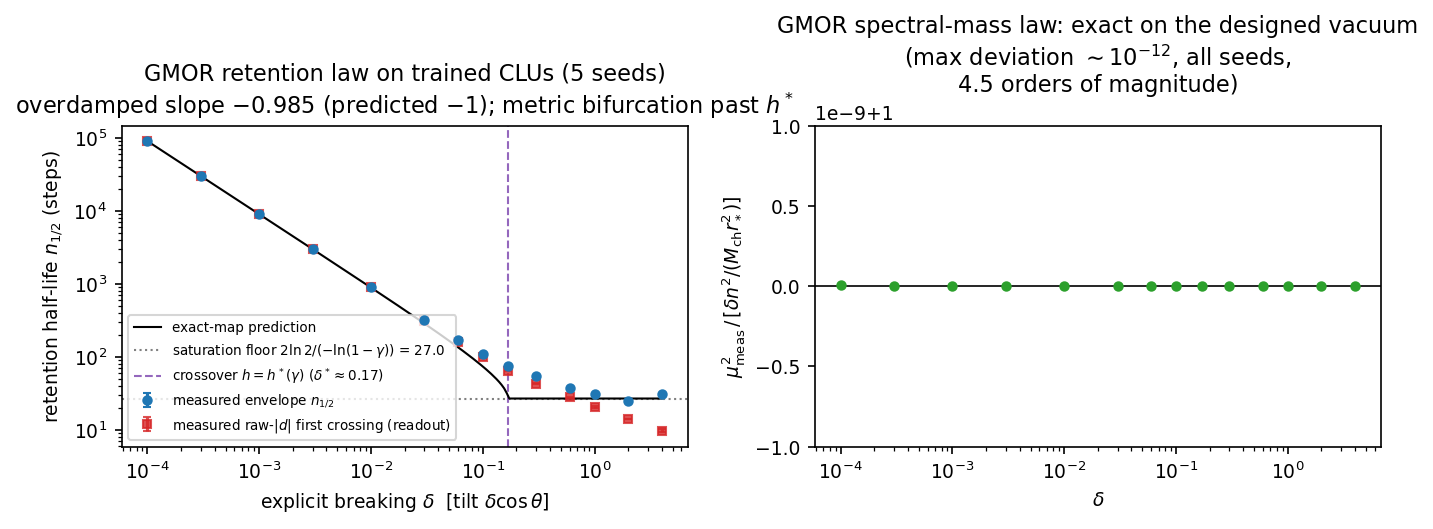
\includegraphics[width=\linewidth]{figs/fig1_gmor.png}
\caption{The retention price list, verified on trained checkpoints. Left: The retention half-life $n_{1/2}$ against the analytic tilt $\delta$. The overdamped branch tracks the predicted law at a fitted slope of $-0.985$ (predicted $-1$) before saturating past $h=h^*(\gamma)$ at the curvature-independent floor of $27.03$ steps ($\gamma=0.05$). Envelope half-life (circles) and raw first-crossing time (squares) diverge after the crossover exceptional point. Right: The curvature identity holds flat at $1.000000\pm5\times10^{-12}$ across $4.5$ decades of $\delta$. \emph{Setup: Trained designed checkpoints, analytic tilts, $5$ seeds, dim $4$, $\gamma=0.05$.}}
\label{fig:pricelist}
\end{figure}

\subsection{Evidence: a published lifetime estimator is the price list's overdamped face}\label{sec:headtohead}

An established retention model should accurately predict independent metrics of decay. \emph{To evaluate this, we apply a recently posted lifetime estimator unchanged onto our trained models.}

The equivariant-Lyapunov preprint (arXiv:2605.03338) isolates a finite memory lifetime using a single-exponential estimator driven by a Lyapunov exponent (inverse time). Our formulation utilizes potential curvature (inverse time squared). We map these directly by executing their exact code-level protocol (phase $0.35$ rad, threshold $0.2$ rad, censoring cap $15000$ steps) over our $5$ trained models across $14$ breaking magnitudes. In the overdamped regime, the measured-to-predicted ratio ranges from $1.012\pm0.000$ to $1.029\pm0.001$, closely matching their reported median of $1.013$.

\emph{However}, this estimator functions exclusively as the overdamped face of our framework ($\mathrm{corr}(\log\mathrm{pred},\log\mathrm{meas})=0.9987$, overdamped-only). The independent predictor fails predictably above the exceptional point crossover, mispredicting by $\approx3.2\times$ at the deepest trained-model breaking ($\delta=4$), exhibiting a $2.202\pm0.155$ delay spike at the crossover, and declining to $0.309\pm0.012$ deep in the underdamped regime. This failure direction is highly calculable. On exact analytic maps, this divergence extends to $\approx5\times$. This represents theoretical containment rather than conflict: our framework recovers their findings below $h^*$ and correctly models the regime structure (floor, ringing, exceptional point) above it, which standard first-order dynamical systems inherently miss.

\begin{figure}[htbp]\centering
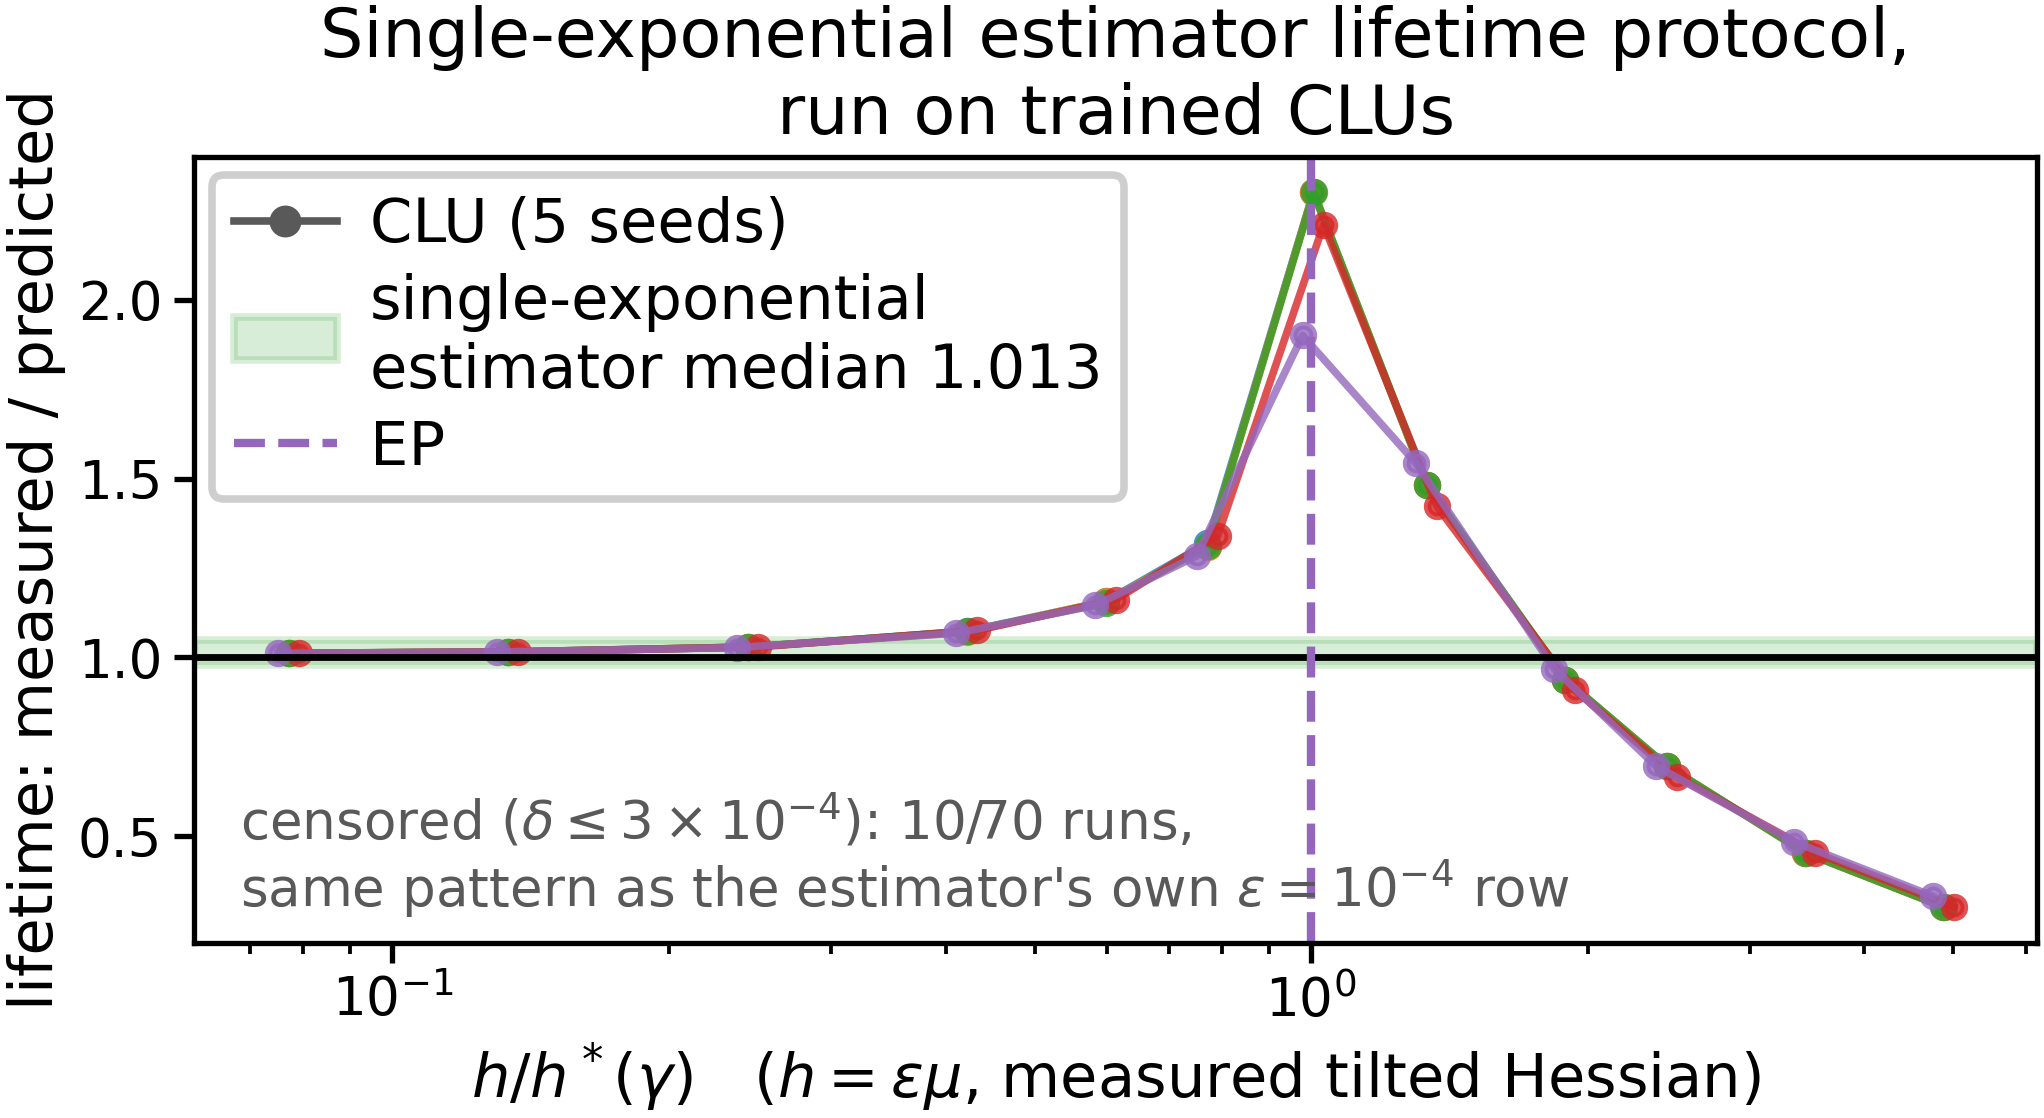
\includegraphics[width=\linewidth]{figs/fig_lifetime_headtohead.png}
\caption{The single-exponential lifetime estimator from arXiv:2605.03338, run unchanged on trained checkpoints, acts as the overdamped face of the transverse-curvature price list. The ratio of measured to predicted lifetime versus breaking magnitude shows containment ($\approx1$) in the overdamped regime. It exhibits a $2.2\times$ delay spike at the exceptional point and degrades to $0.31\times$ underdamped, validating the bounded limits of first-order single-exponential estimation.}
\label{fig:lifetime_headtohead}
\end{figure}

\subsection{The honest negative: where the price list does not extend}\label{sec:boundary}

It is often assumed that symmetric training data naturally induces flat geometric directions. \emph{Unlike structural constraints, we find that training data alone does not achieve this on this architecture class.}

A generic MLP potential trained on symmetric data develops softest emergent curvatures of $\mu^2=5.1/5.9/5.4\!\times\!10^{-2}$ across $3$ seeds. Compared to the designed flat mode ($\le2.4\!\times\!10^{-15}$), this presents a gap of $13$--$14$ orders of magnitude. Operationally, this emergent arm functions not on a continuum, but on discrete washboard minima ($\approx1$--$1.6$ bits capacity), where any continuous written coordinate $\delta$ fully relaxes. While the damping-optimum retention law mathematically holds here, the continuous coset register itself is strictly a designed feature.

\paragraph{Autonomous retention against learned baselines.} Gated and oscillatory recurrent networks reliably minimize task error. \emph{However, fitting the task does not equate to holding the continuous state autonomously.} We write a latent phase into optimized baseline models (LSTM, LEM, and coRNN trained with learning rate sweeps) and allow them to run autonomously without input. The structural triad---the exact latch, the $\mu^{-2}$ scaling law, and the bounded coordinate motion---is completely absent in these baselines. Under autonomous execution, coRNN, LEM, and LSTM lose the stored analog phase within $\approx5.6/56/69$ map-steps, respectively, with coordinates randomizing beyond $1.2$ rad. In contrast, the generically-trained symplectic unit holds for $\approx263$ map-steps with strictly bounded coordinate motion ($\approx0.35$ rad). Crucially, the designed unit never drifts across all $5$ seeds.

\paragraph{Honest compute gap.} We emphasize that the raw $263$-to-$69$ map-step advantage does not survive normalized compute analysis. We explicitly retire it as a wall-time efficiency claim. A single Verlet update costs $\approx6.2\times$ the wall time of an LSTM cell and $\approx3.1\times$ that of a LEM cell ($\approx14$--$15\times$ FLOPs). When normalized per unit of retention, our architecture demands significantly more computational overhead (Appendix~\ref{app:compute}).

\subsection{The price list survives the training-time correction}\label{sec:cure}

A structural retention advantage is functionally useless if the training objective actively erodes the required potential landscape. \emph{In our system, standard contrastive divergence explicitly destroys the continuous register.}

Wake--sleep contrastive divergence drives the order parameter $r^*$ to zero. At $1000$ epochs, the designed vacuum inverts in $8/8$ runs, eliminating the orbit and generating invariant minimisers with strictly positive $\mu^2$. This represents a manifestation of the fine-tuning problem, where the training objective acts as the primary perturbation. To resolve this, we anchor the condensate using a $V(\text{data})$ energy anchor ($\lambda=100$). Over $5$ seeds, the anchor maintains $r^*=0.911\pm0.016$, trading off weaker noise rejection and a higher wake MSE. \emph{Therefore, we report that the transverse-curvature price list survives this corrective intervention.} Across $3000$ anchored epochs ($\approx20\times$ the baseline erosion horizon), the retention laws remain entirely intact (Appendix~\ref{app:anchor}). The curvature ratio holds to $1.5\!\times\!10^{-12}$, the slope holds at $-0.956$ (the per-point fit over all overdamped rows), the floor remains unchanged, and the exceptional-point onset is bit-identical at $0.5165$.

\section{Discussion}\label{sec:discussion}

\begin{itemize}
    \item \textbf{Operational Scope:} Measurements rely on a laptop CPU, dimension $4$, the $S^1$ testbed, and $\le5$ seeds.
    \item \textbf{Analytical Limits:} The solvable core is quadratic. Trained measurements remain localized to the critical points of $V_\theta$. Finite-$T$ diffusion laws are exclusively bounded by fluctuation--dissipation theorem constraints.
    \item \textbf{Task Benchmarking:} We do not claim external task benchmark superiority. \emph{No external benchmark is won on its own headline metric anywhere in this paper.} Evaluative comparisons utilize autonomous diagnostic protocols on synthetic topologies to isolate structural retention.
    \item \textbf{Off-Distribution Stability:} BIBO stability bounds apply only to the autonomous, designed setting. We make no claims regarding input-driven off-distribution stability on trained networks.
    \item \textbf{Substrate Scope:} Stated once, in our own voice: these laws govern the store; end-to-end performance additionally depends on the encoder, measured separately, with its parameter and state-byte budget ledgered.
\end{itemize}

By quantifying this price list, we shift the operational perspective on flat directions. A trained memory network is best interpreted as a composite of exact latches (symmetry-protected moduli of $V_\theta$) and tunable registers (nearly-flat modes bounded by $\mu^2$). Kinetic isotropy acts as the price for an equivariant write current, rather than the register itself. Promising future directions include measuring the $\mu^{-2}$ crossover and floor at latent dimensions $\gtrsim64$ (where mode mixing may complicate the reduction), analyzing solution degeneracy between the designed and emergent arms, integrating equivariant-control wrappers for supervised tasks, and generalizing the price list beyond abelian $SO(2)$ to non-abelian tori constructions.

\section*{References}
\begingroup
\setlength{\parindent}{-0.22in}\setlength{\leftskip}{0.22in}\setlength{\parskip}{\smallskipamount}

Aitken, K., Garrett, M., Olsen, S., \& Mihalas, S. (2022). The geometry of representational drift in natural and artificial neural networks. \emph{PLOS Computational Biology} 18(11):e1010716.

Akhtiamov, D., \& Thomson, M. (2023). Connectedness of loss landscapes via the lens of Morse theory. \emph{PMLR} 197:171--181.

Anonymous (2026). \emph{The theory note}: an exactly-solvable theory of retention, latching and forgetting for damped symplectic recurrences. Provided in the supplementary material.

Aslan, B., Platt, D., \& Sheard, D. (2023). Group invariant machine learning by fundamental domain projections. \emph{PMLR} 197:181--218.

Behrouz, A., Zhong, P., \& Mirrokni, V. (2025). Titans: Learning to memorize at test time. \emph{NeurIPS 2025}. arXiv:2501.00663.

Burak, Y., \& Fiete, I. R. (2012). Fundamental limits on persistent activity in networks of noisy neurons. \emph{PNAS} 109(43):17645--17650.

Csord\'as, R., \& Schmidhuber, J. (2019). Improving differentiable neural computers through memory masking, de-allocation, and link distribution sharpness control. \emph{ICLR 2019}. arXiv:1904.10278.

Di Bernardo, A., Valente, A., Mastrogiuseppe, F., \& Ostojic, S. (2025). Shaping manifolds in equivariant recurrent neural networks. arXiv:2511.04802.

Dinc, F., Cirakman, E., Kurtkaya, B., Yuksekgonul, M., Jiang, Y., Schnitzer, M. J., \& Tanaka, H. (2025). A ghost mechanism: An analytical model of abrupt learning in recurrent networks. arXiv:2501.02378.

D\"onmez, A. (2024). Discovering latent causes and memory modification: A computational approach using symmetry and geometry. \emph{PMLR} 228.

Driscoll, L. N., Pettit, N. L., Minderer, M., Chettih, S. N., \& Harvey, C. D. (2017). Dynamic reorganization of neuronal activity patterns in parietal cortex. \emph{Cell} 170(5):986--999.e16.

Fischer, A., \& Igel, C. (2010). Empirical analysis of the divergence of Gibbs-sampling-based learning algorithms for restricted Boltzmann machines. \emph{ICANN 2010}, LNCS 6354:208--217.

Gardner, R. J., et al. (2022). Toroidal topology of population activity in grid cells. \emph{Nature} 602(7895):123--128.

Golubitsky, M., Stewart, I., \& Schaeffer, D. G. (1988). \emph{Singularities and Groups in Bifurcation Theory: Volume II}. Applied Mathematical Sciences 69, Springer.

Graves, A., Wayne, G., \& Danihelka, I. (2014). Neural Turing machines. arXiv:1410.5401.

Graves, A., et al. (2016). Hybrid computing using a neural network with dynamic external memory. \emph{Nature} 538(7626):471--476.

Gu, A., Dao, T., Ermon, S., Rudra, A., \& R\'e, C. (2020). HiPPO: Recurrent memory with optimal polynomial projections. \emph{NeurIPS 2020}. arXiv:2008.07669.

Hairer, E., Lubich, C., \& Wanner, G. (2006). \emph{Geometric Numerical Integration} (2nd ed.). Springer Series in Computational Mathematics 31.

Haputhanthri, U., et al. (2025). Understanding and controlling the geometry of memory organization in RNNs. arXiv:2502.07256.

Hinton, G. E., Dayan, P., Frey, B. J., \& Neal, R. M. (1995). The ``wake-sleep'' algorithm for unsupervised neural networks. \emph{Science} 268(5214):1158--1161.

Hochreiter, S., \& Schmidhuber, J. (1997). Long short-term memory. \emph{Neural Computation} 9(8):1735--1780.

Huang, A., Singh, S. H., Martinelli, F., \& Rajan, K. (2025). Measuring and controlling solution degeneracy across task-trained recurrent neural networks. \emph{NeurIPS 2025}. arXiv:2410.03972.

Iqbal, N., Keller, T. A., Song, Y., Miyato, T., \& Welling, M. (2026). Spontaneous symmetry breaking and Goldstone modes for deep information propagation. arXiv:2605.14685.

Jawahar, P., \& Pierini, M. (2026). CHLU: The causal Hamiltonian learning unit as a symplectic primitive for deep learning. arXiv:2603.01768.

Jelassi, S., Brandfonbrener, D., Kakade, S. M., \& Malach, E. (2024). Repeat after me: Transformers are better than state space models at copying. \emph{ICML}, PMLR 235:21502--21521.

Jude, J., Perich, M. G., Miller, L. E., \& Hennig, M. H. (2023). Capturing cross-session neural population variability through self-supervised identification of consistent neuron ensembles. \emph{PMLR} 197:234--257.

Karuvally, A., Lertsaroj, P., Sejnowski, T. J., \& Siegelmann, H. T. (2025). Exponential dynamic energy network for high-capacity sequence memory (EDEN). \emph{NeurIPS 2025}. arXiv:2510.24965.

Keller, T. A. (2025). Flow equivariant recurrent neural networks. \emph{NeurIPS 2025}. arXiv:2507.14793.

Khona, M., \& Fiete, I. R. (2022). Attractor and integrator networks in the brain. \emph{Nature Reviews Neuroscience} 23:744--766.

Kim, S. S., Rouault, H., Druckmann, S., \& Jayaraman, V. (2017). Ring attractor dynamics in the \emph{Drosophila} central brain. \emph{Science} 356(6340):849--853.

Kong, L.-W., Brewer, G. A., \& Lai, Y.-C. (2024). Reservoir-computing based associative memory and itinerancy for complex dynamical attractors. \emph{Nature Communications} 15:4840.

Krupa, M. (1990). Bifurcations of relative equilibria. \emph{SIAM Journal on Mathematical Analysis} 21(6):1453--1486.

Lillemark, H. J., Huang, B., Zhan, F., Du, Y., \& Keller, T. A. (2026). Flow equivariant world models: Memory for partially observed dynamic environments. arXiv:2601.01075.

McLachlan, R. I., \& Perlmutter, M. (2001). Conformal Hamiltonian systems. \emph{Journal of Geometry and Physics} 39(4):276--300.

Mo, H. H. (2026). Symmetry-protected Lyapunov neutral modes in equivariant recurrent networks. arXiv:2605.03338.

Nijkamp, E., Hill, M., Han, T., Zhu, S.-C., \& Wu, Y. N. (2020). On the anatomy of MCMC-based maximum likelihood learning of energy-based models. \emph{AAAI 2020}. arXiv:1903.12370.

Ramsauer, H., et al. (2021). Hopfield networks is all you need. \emph{ICLR 2021}. arXiv:2008.02217.

Renart, A., Song, P., \& Wang, X.-J. (2003). Robust spatial working memory through homeostatic synaptic scaling in heterogeneous cortical networks. \emph{Neuron} 38(3):473--485.

Rumberger, M. (2001). Lyapunov exponents on the orbit space. \emph{Discrete and Continuous Dynamical Systems} 7(1):91--113.

Rusch, T. K., \& Mishra, S. (2021a). Coupled oscillatory recurrent neural network (coRNN). \emph{ICLR 2021}. arXiv:2010.00951.

Rusch, T. K., \& Mishra, S. (2021b). UnICORNN: A recurrent model for learning very long time dependencies. \emph{ICML}, PMLR 139:9168--9178.

Rusch, T. K., Mishra, S., Erichson, N. B., \& Mahoney, M. W. (2022). Long expressive memory for sequence modeling. \emph{ICLR 2022}. arXiv:2110.04744.

S\'agodi, \'A., Mart\'in-S\'anchez, G., Sokó\l, P., \& Park, I. M. (2024). Back to the continuous attractor. \emph{NeurIPS 2024}. arXiv:2408.00109.

Seung, H. S. (1996). How the brain keeps the eyes still. \emph{PNAS} 93(23):13339--13344.


Tieleman, T. (2008). Training restricted Boltzmann machines using approximations to the likelihood gradient. \emph{ICML 2008}, 1064--1071.

Vafidis, P., Owald, D., D'Albis, T., \& Kempter, R. (2022). Learning accurate path integration in ring attractor models. \emph{eLife} 11:e69841.

van der Ouderaa, T. F. A., \& van der Wilk, M. (2023). Sparse convolutions on Lie groups. \emph{PMLR} 197:48--62.

Vastola, J. (2024). Optimal packing of attractor states in neural representations. \emph{PMLR} 228:425--442.

Wang, B., \& Ponce, C. R. (2023). On the level sets and invariance of neural tuning landscapes. \emph{PMLR} 197:278--300.

Xu, D., Gao, R., Zhang, W.-H., Wei, X.-X., \& Wu, Y. N. (2023). Conformal isometry of Lie group representation in recurrent network of grid cells. \emph{PMLR} 197:370--387.
\endgroup

\appendix

\section{The laws survive the training-time correction}\label{app:anchor}

\begin{figure}[htbp]\centering
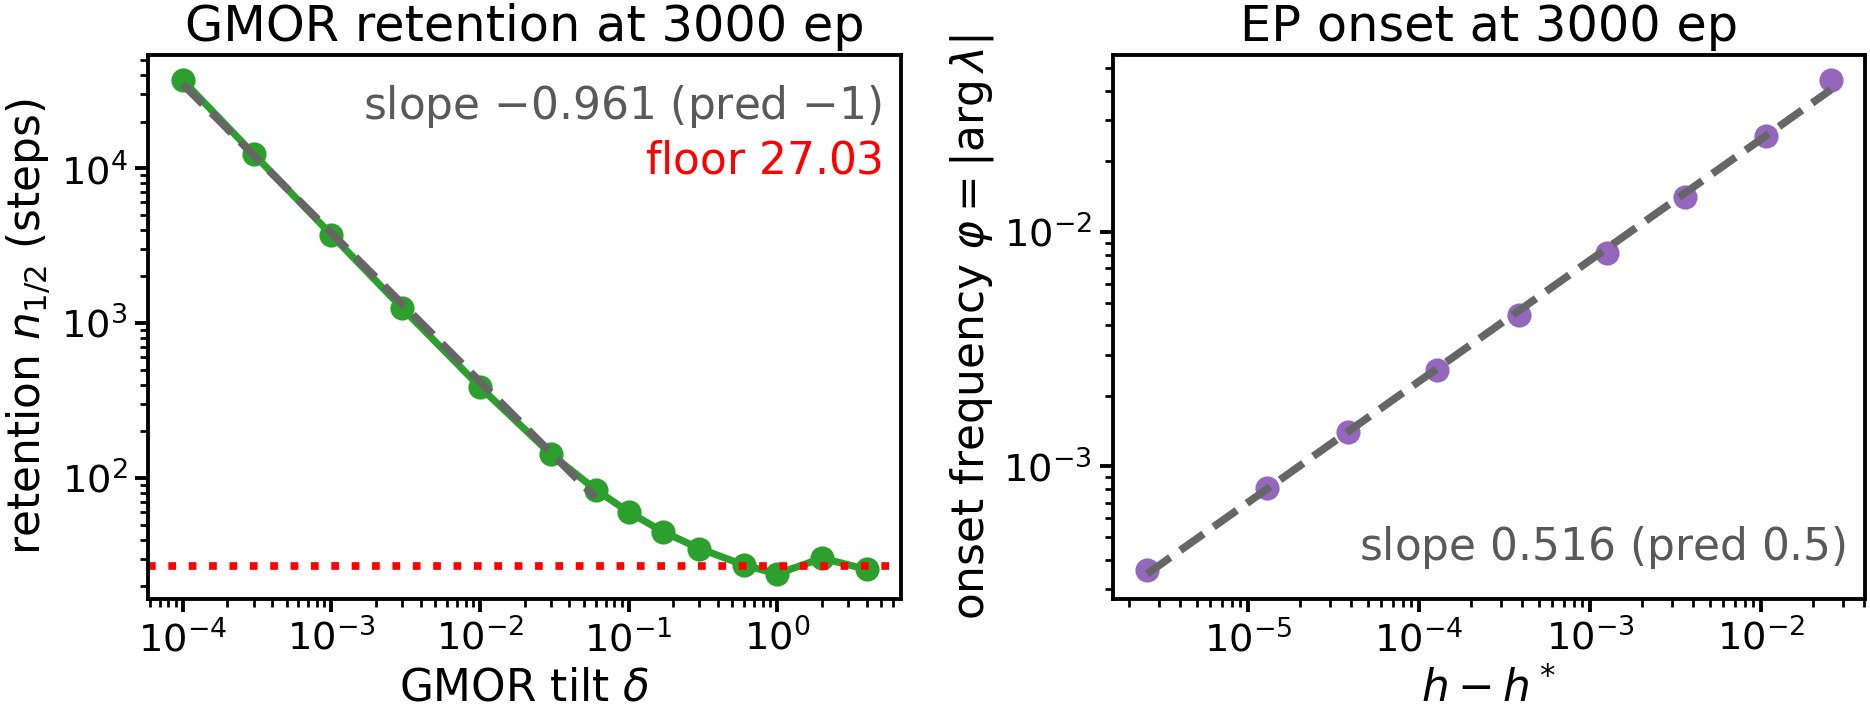
\includegraphics[width=\linewidth]{figs/fig2_anchor_cure_laws.png}
\caption{The foundational retention laws of the price list survive the applied anchor correction at $3000$ epochs ($\approx20\times$ the erosion horizon; anchored $\lambda=100$, $3$ seeds). Left: The retention law $n_{1/2}$ versus tilt $\delta$ demonstrates anchored points tracking the predicted slope (fitted $-0.961$ against predicted $-1$; the seed-mean OLS over the $7$ overdamped $\delta$) before saturating at the curvature-independent floor of $27.03$. The $\mu^2/\delta$ ratio maintains $1.0000\pm10^{-12}$ stability over $4.6$ decades. Right: The exceptional-point onset follows $\varphi\propto\sqrt{h-h^*}$ above the critical threshold, with a fitted slope of $0.516$ (predicted $0.5$) and exactly $\varphi=0$ below, remaining bit-identical to the baseline $150$-epoch measurement. \emph{Results map to a designed testbed under the applied cure, providing structural evidence that the recipe maintains integrity through erosive training scales.}}
\label{fig:sf3}
\end{figure}

\section{The explicit price of the physical prior}\label{app:loan}

We explicitly clarify that this section analyzes the baseline cost of embedding physics priors and does not serve as a primary performance claim.

Evaluating the system against parameter-matched controls (dimension $4$, $150$ epochs, $\pm0.05\%$ parameters, $3$ seeds, identical MLP potential) reveals a strict Pareto tradeoff. Conserving phase-space volume inherently provides bounded (BIBO) dynamics inside the coercive-potential scope ($1.00$ versus $0.33$ for the broken-volume baseline), protects a near-flat direction ($\mu^2=0.008$ versus $0.122$), and enables vacuum survival under contrastive-divergence training ($r^*=0.72$ versus $0$). \emph{However}, this strict prior fundamentally constrains raw fitness. An unconstrained twin achieves an evaluation MSE of $0.0128$, outperforming the constrained unit's $0.190$. This penalty is proven mathematically to be contraction-forbidden by the volume conservation axiom, as the broken-volume baseline precisely recovers $\approx2.4\times$ of the performance gap purely by leaking volume.

The constrained model's primary asset is bounded execution by construction, not achieving the lowest steady-state MSE. While the twin model's raw fit diverges dramatically after $\approx700$ steps (reaching an MSE of $196$ at $5000$ steps), the physically-informed unit maintains a bounded plateau of $\approx0.20$--$0.23$. Only global damping mechanisms recover the lost fit; introducing a learned friction field does not functionally substitute.

\emph{Data configuration: Dimension $4$, hidden $64$, learned-Newtonian kinetic term, $\mathrm{dt}=0.05$, circle $R=1\times256$, $150$ epochs, $3$ seeds, wake-only objective except the $\gamma_\phi$ rung. Cumulative fit MSE against horizon is measured on the stationary circle-vacuum orbit, parameter-matched to $\pm0.2\%$ (CLU $4549$ / broken-volume $4557$ / twin $4551$).}

\begin{center}
\begin{tabular}{lcccc}
\toprule
Horizon (steps) & \textbf{Twin} & \textbf{CLU} & Broken-Volume & LSTM \\
\midrule
$10$ & $\mathbf{2.9{\times}10^{-6}}$ & $2.2{\times}10^{-5}$ & $1.1{\times}10^{-4}$ & $7.5{\times}10^{-2}$ \\
$50$ & $\mathbf{6.2{\times}10^{-5}}$ & $1.2{\times}10^{-3}$ & $1.0{\times}10^{-3}$ & $4.9{\times}10^{-2}$ \\
$100$ & $\mathbf{2.4{\times}10^{-4}}$ & $1.2{\times}10^{-2}$ & $4.1{\times}10^{-3}$ & $4.9{\times}10^{-2}$ \\
$500$ & $\mathbf{1.1{\times}10^{-2}}$ & $1.8{\times}10^{-1}$ & $9.7{\times}10^{-2}$ & $7.7{\times}10^{-2}$ \\
$1000$ & $3.2{\times}10^{-1}$ & $\mathbf{2.0{\times}10^{-1}}$ & $1.2{\times}10^{-1}$ & $9.9{\times}10^{-2}$ \\
$5000$ & $1.96{\times}10^{2}$ & $2.2{\times}10^{-1}$ & $\mathbf{1.4{\times}10^{-1}}$ & $1.3{\times}10^{-1}$ \\
\bottomrule
\end{tabular}
\end{center}

\emph{We emphasize that the following table represents an independent wake-only experiment. The absolute MSE scale and its associated twin ($0.0047$) are not mathematically cross-comparable with the prior parameter-matched table (twin $0.0128$) due to variations in seeds and training objectives. Comparisons must remain restricted to intra-table relative ratios.}

\begin{center}
\begin{tabular}{lccccc}
\toprule
Model Variant & Eval MSE & \% Gap Recovered & BIBO & Latch Drift & Flat $\mu^2$ \\
\midrule
Twin (No Physics) & $0.0047$ & $100\%$ (Ref) & $1.00$ & --- & --- \\
CLU Conservative ($\gamma=0$) & $0.2066$ & $0\%$ (Ref) & $1.00$ & $0.778$ & $5.2{\times}10^{-3}$ \\
$+\gamma$ Global ($\gamma=0.05$) & $0.0216$ & $\mathbf{92\%}$ & $1.00$ & $0.778$ & $5.2{\times}10^{-3}$ \\
$+\gamma_\phi$ Learned Field ($K=2$) & $0.2548$ & $-24\%$ & $1.00$ & $0.706$ & $2.1{\times}10^{-2}$ \\
\bottomrule
\end{tabular}
\end{center}

\section{The autonomous-retention head-to-head against learned baselines}\label{app:retention}

\begin{figure}[htbp]\centering
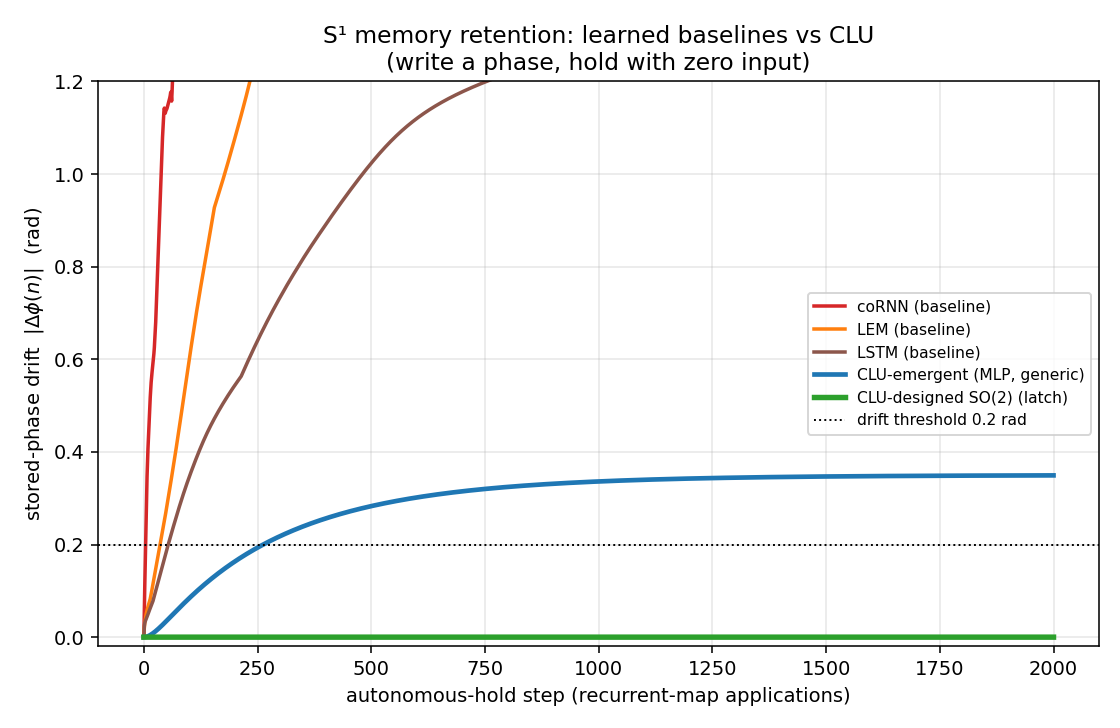
\includegraphics[width=\linewidth]{figs/fig3_retention_overlay.png}
\caption{Autonomous retention evaluated via the $S^1$ protocol (arXiv:2605.03338). A designated phase is encoded, the input is systematically removed, and structural drift of the stored phase is tracked continuously across unspooled map applications. The learned baselines exhibit critical phase loss within $\approx5.6/56/69$ map-steps (coRNN/LEM/LSTM) as the latent coordinate completely randomizes beyond $1.2$ rad. In contrast, the generically-trained symplectic unit maintains a bounded state of $\approx0.35$ rad, and the symmetry-designed unit registers strictly zero drift. Baseline and emergent measurements represent the median across $5$ and $3$ seeds respectively, while the designed curve is a single representative checkpoint---the $5/5$-seed latch statement is Sec.~\ref{sec:boundary}'s, not this figure's. Experimental constraints: Dimension $4$, hidden $64$, single-core CPU execution, drift threshold defined at $0.2$ rad, evaluated at deterministic $T=0$.}
\label{fig:retention}
\end{figure}

\section{Per-step compute requirements}\label{app:compute}

We document the explicit performance normalization factoring that necessitates our retirement of the naive ``map-step'' claim as a formal metric of compute efficiency. Measured strictly on a single-core CPU via f32 XLA, one CLU dissipative-Verlet step entails two $\nabla_qV$ backpropagations through a $\dim 4\to64\to64\to1$ tanh MLP with a learned-Newtonian kinetic term. Wall time is the median of $7$ scan-amortized repetitions over $2{\times}10^5$ steps; the na\"ive single-call timing is dispatch-bound at a $\approx5\,\mu$s floor and is \emph{not} reported.

\begin{center}
\begin{tabular}{lccc}
\toprule
Unit Configuration & Parameters & FLOPs/Step & Wall ns/step \\
\midrule
CLU Verlet (h$64$, dim $4$, KDK) & $4549$ & $\mathbf{36148}$ & $1554$ \\
LSTM cell (h$16$) & $1186$ & $2512$ & $252$ \\
LEM cell (h$16$) & $1186$ & $2400$ & $500$ \\
\bottomrule
\end{tabular}
\end{center}

\begin{center}
\begin{tabular}{lcc}
\toprule
Normalization Standard & CLU vs.\ LSTM & CLU vs.\ LEM \\
\midrule
Raw map-steps ($263$ vs.\ $69$/$56$) & $3.8\times$ longer & $4.7\times$ longer \\
FLOP-normalized & $\mathbf{54.8\times}$ more & $\mathbf{70.7\times}$ more \\
Wall-normalized & $\mathbf{23.5\times}$ more & $\mathbf{14.6\times}$ more \\
\bottomrule
\end{tabular}
\end{center}

\textbf{Confound, flagged:} the comparison is not width-matched, CLU at hidden $64$ with two gradient evaluations against baselines at hidden $16$; a width-matched CLU would narrow the gap, but the sign is robust because the Verlet step requires two potential backpropagations, and the $263/69/56$ retention numbers come from these specific configurations. The measurement is single-core CPU at batch $1$; GPU or batched throughput could shift the wall ratios, though not the FLOPs.

\section{Documented negative results and formal limitations}\label{app:neg}

We structurally record all hypothesis failures and architectural limitations evaluated during this work.

\begin{center}
\begin{tabular}{@{}p{1.52in} p{1.52in} p{2.06in}@{}}
\toprule
Tested Hypothesis & Operational Result & Supporting Measurement \\
\midrule
Does a learned inertial mass isotropize strictly on symmetric data? &
No. The breaking is fundamentally invisible to the standard Hessian and the latch, appearing only as bounded Noether-charge oscillations. &
Log-mass split ratios are $0.98$ / $1.18$ / $5.4$ from init to $150$ ep; charge amplitudes $5.4/1.6/0.082{\times}10^{-2}$; tied controls exactly $1.0000$. \\[2pt]
Does wake--sleep contrastive divergence preserve designed degenerate vacua? &
No. It strictly inverts it. A $V(\text{data})$ energy anchor must be introduced to stabilize it. &
$r^*\to0$ across $8/8$ iterations at $1000$ ep; inversion at epoch $116$/$442$/$959$ by sleep frequency; anchor $\lambda{=}100$ successfully holds $5/5$ seeds at $r^*{=}0.911\pm0.016$. \\[2pt]
Does an emergent (MLP) unit maintain a continuous coset register? &
No. The continuous framework is strictly designed. Emergent variations resolve to discrete washboard minima configurations. &
$1-|\lambda_{\rm coset}|\approx10^{-3}$ against the designed $\le1.1{\times}10^{-15}$, $\sim\!12$ orders; written $\delta$ retained $\le2.1{\times}10^{-3}$; capacity $\approx1$--$1.6$ bits. \\[2pt]
Can explicit-breaking coefficients function as reliable lifetime dials on learned stores? &
No. Increasing the breaking magnitude inversely lowers the softest eigenvalue, and absolute coercivity dictates the ceiling limit. &
$\lambda_{\min}$ ranges $+0.0994\to-8.2846$ and $+0.3291\to-1.1980$ over four decades of breaking; hard operational ceiling observed at $\tau_{\max}=\Gamma/2\alpha=4.0$; tilt-vacuum residual $0.140$--$0.343$ against a random-direction baseline $1/\mathrm{dim}=0.167$. \\[2pt]
Is the coded momentum-coupled Langevin sampler FDT-exact across all kinetic modes? &
No. It proves FDT-exact strictly in Newtonian execution. Under relativistic operations, no noise scale converges the chain to a Gibbs invariant. &
Required per-mode scale verified as $\sigma^\star_i=\sqrt{M_iT\gamma(2-\gamma)}$. \\[2pt]
Can this unit enter the input-driven path-integration task-RMSE axis? &
No. It has no native velocity ingestion and the equivariant-control wrapper is unbuilt. No task-RMSE was fabricated. &
--- \\[2pt]
\bottomrule
\end{tabular}
\end{center}

\begin{center}
\begin{tabular}{@{}p{1.52in} p{1.52in} p{2.06in}@{}}
\toprule
Tested Hypothesis & Operational Result & Supporting Measurement \\
\midrule
Do raw $n_{1/2}$ exponents discriminate designed from emergent stores? &
No. Instrument, not physics: a matched designed control on the same grid gives the same slopes, both carrying the $\ell_\theta/\Delta$ boundary layer. No $n_{1/2}$ may be quoted without its $\Delta$ and $\ell_\theta/\Delta$. &
Designed control $\mathrm{d}\log n_{1/2}/\mathrm{d}\log T=-0.53,-0.60,-1.04$ and $\mathrm{d}\log n_{1/2}/\mathrm{d}\log\gamma=+0.78,+0.63,+0.55$; $\ell_\theta/\Delta$ up to $2.0$. \\[2pt]
Do a learned friction field and a curvature governor compose usefully? &
No. The pair is Pareto-dominated by either alone, and a learned compact-support gate under-covers without accurate placement. &
Locus discovery $2/6$ before adaptive-$K$, $2/3$ after; best learned rejection $0.861$; a $\lambda$ re-sweep does not approach the oracle. \\[2pt]
Can friction stabilize a saddle, or an energy gate catch isoenergetic escape? &
No to both---a genuine scope limitation of the class. Only curvature control of $V_\theta$ and the mass-anisotropic cap $v_i^{\max}=c/\sqrt{M_i}$ bound expanding or isoenergetic modes. &
$\lambda_+>1$ for all $\gamma$, with $\min_\gamma(\lambda_+-1)=1.4{\times}10^{-5}$. \\[2pt]
Is a mean-spectrum chaos regularizer informative? &
No. It is degenerate; a chaos penalty must use a max or positive-part statistic. &
--- \\[2pt]
Is \texttt{sleep\_temperature} active at \texttt{sleep\_friction=0}? &
No. A silent knob; cite it when reproducing temperature-swept sleep runs. &
$\sigma\propto\sqrt{\gamma_{\rm sleep}}$, so the swept runs are bit-identical. \\
\bottomrule
\end{tabular}
\end{center}

\emph{We clarify specific architectural limitations identified in these negatives:} The closed-form charge-oscillation amplitude bounds strictly dictate on-vacuum-orbit behaviors. Consequently, anisotropic channels continue to latch with mathematically infinite half-lives; mass-tying serves primarily to enforce angle-independent write currents rather than structurally save the register itself. Furthermore, we explicitly emphasize that explicit breaking parameters do not scale linearly with system retention outside of purely designed $SO(2)$ geometric environments.

\textbf{The sampler row's scope, stated precisely, because the qualifier is load-bearing.} The coded damping substep is an additive Gaussian momentum kick of fixed covariance, so the chain's invariant momentum marginal is necessarily Gaussian-smoothed; for a \emph{relativistic} kinetic term the Gibbs momentum marginal is Maxwell--J\"uttner, which is not of that form (\emph{theory note}, Prop-9$'$---a characteristic-function argument needing neither $V=0$ nor linear damping). \textbf{The failure is in the \emph{sampler}, not in the \emph{thermodynamics}}: the configurational equilibrium $\pi_q\propto e^{-V_\theta/T}$ is relativity-insensitive, since the momentum integral factorizes out, so a relativistic unit's equilibrium distribution is perfectly well-defined and the chain simply fails to sample it; a one-line thermostat carrying a randomized, momentum-dependent inertia equal to the relativistic mass repairs it. We therefore never assert that a relativistic unit ``has no equilibrium''. \textbf{This touches no result in this paper:} the trained units here are \texttt{newtonian\_learned} throughout, so $\sigma^\star$ is exact for every configuration we run---the qualifier is a \emph{scope clause} on a class-level theorem, not a correction to a measurement.

\section{Contextualizing prior work boundaries}\label{app:pos}

To ensure precise attribution and clearly demarcate the novelty of our contributions, we explicitly contextualize our methods against closely associated literature:

\begin{enumerate}
    \item \textbf{Retention Guarantees in State-Space Models:} Architectures such as HiPPO-LegS (Gu et al.\ 2020) maintain $O(tL/\sqrt N)$ retention guarantees, utilizing exact timescale equivariance devoid of discrete tuning boundaries. We do not assert that our $\mu^2$-driven continuous curvature spectra out-perform these bounds natively.
    \item \textbf{Retrieval as Rollout:} Treating continuous retrieval sequences as deterministic dynamical rollouts is fully established by Kong, Brewer \& Lai (2024). Our implementation builds on this by enforcing strict symplecticity and Hamiltonian constraints.
    \item \textbf{Continuity as a Novelty:} The foundational mechanics of continuous and soft-memory mapping are native to the Neural Turing Machine (Graves et al.\ 2014) and DNC lineages. Key/value entanglement phenomena diagnosed in these models (Csord\'as \& Schmidhuber 2019) technically map onto our architecture, though our evaluation focuses strictly on geometric state drift.
    \item \textbf{Transformer Scaling Comparisons:} The frameworks explored in this paper are analytically bounded tools ($1$--$1.6$ bits per emergent register). We make no claims regarding benchmark scaling or general superiority against current Transformer implementations.
\end{enumerate}

\textbf{The head-to-head reproduced on the preprint's own instrument.} Sec.~\ref{sec:headtohead}'s result does not depend on substituting the exact Jacobian gap for the preprint's predictor. With the preprint's own finite-horizon estimator $\hat\lambda(T{=}128)$ the result holds on that instrument: $\mathrm{corr}=0.9995$ overdamped, meas/pred $0.86$--$1.03$, and $0.30$ at $\delta=4$ against the exact-gap $0.31$.

\section{GMOR verification on trained checkpoints}\label{app:gmor}

\emph{Data configuration: Designed testbed mapped with analytic tilts and an analytic spurion to verify the theory's exactness. Evaluated on $5$ primary seeds at $150$ epochs and $3$ anchored seeds at $3000$ epochs, dimension $4$, executed on CPU with $f64$ probes and zero network retraining. \textbf{GMOR proper---G.3 onward---is demoted from the main text and retained here in full; it is a supporting result, not one of this paper's claims.}}

\textbf{G.1 The foundational retention scaling law.} The retention scaling law $n_{1/2}\propto\mu^{-2}$ functions analytically as a Gell-Mann--Oakes--Renner (GMOR) relationship within the spectral mass context ($\mu^2F^2=\delta\Sigma$). Over $70$ distinct tilt rows mapped across a machine-flat trained vacuum, the constitutive identity aligns to $3.2{\times}10^{-10}$. Across $4.5$ decades, the scaling curvature ratio holds to $1.000000\pm5{\times}10^{-12}$. The $\sqrt{h-h^*}$ onset holds down to $h-h^*=2.6{\times}10^{-6}$ on a fine multiplicative grid ($h-h^*\in[-4.2{\times}10^{-3},2.6{\times}10^{-2}]$). Where the quality factor permits ($f=2,4$), the trajectory frequency matches the Jacobian frequency to $0.06$--$0.3\%$; near onset the mode decays before one period completes, so the exceptional point is spectroscopically real but dynamically silent there.

\textbf{G.2 Secondary bounds of the damping corollary.} Modulating the damping constant $\gamma$ at a fixed spectral mass yields a distinctly non-monotone retention profile. The function $n_{1/2}(\gamma)$ forms a V-shaped curve, identifying its minimum directly beneath the exact critical-damping value $\gamma^*\approx2\varepsilon\mu$. Consequently, an isolated evaluation of retention scaling at a single $\gamma$ remains technically uninformative regarding the functional sign of $\partial n_{1/2}/\partial\gamma$ unless its position relative to the damping critical threshold is analytically specified.

\textbf{G.3 Ambient spurion integration.} To disentangle the radial dependence masked by simple angular tilts ($V\to V+\delta(1-\cos n\theta)$), we introduce a linear ambient spurion ($V\to V-\delta\,(u\cdot q)$). Under this condition, the vacuum radius dynamically tracks with $\delta$, allowing explicit and separate verification of the pseudo-Goldstone spectral mass ($\mu^2$), the decay constant ($F^2$), and the condensate ($\Sigma$). Across $8$ trained checkpoints mapped from $\delta\in[10^{-8},0.3]$, the absolute deviation between $\mu^2F^2$ and $\delta\Sigma$ is structurally bounded by $\max|\mu^2F^2-\delta\Sigma|=1.33{\times}10^{-15}$.

\textbf{G.4 Condensate tracking.} Evaluated via geometric parameterizations, Hellmann--Feynman theorem proofs, and finite difference differentials, the running condensate $\Sigma$ scales by $+16.1\%$ to $+210.1\%$ across the full evaluated $\delta$ grid, operating entirely blind to the natively shipped angular tilt functions.

\begin{figure}[htbp]\centering
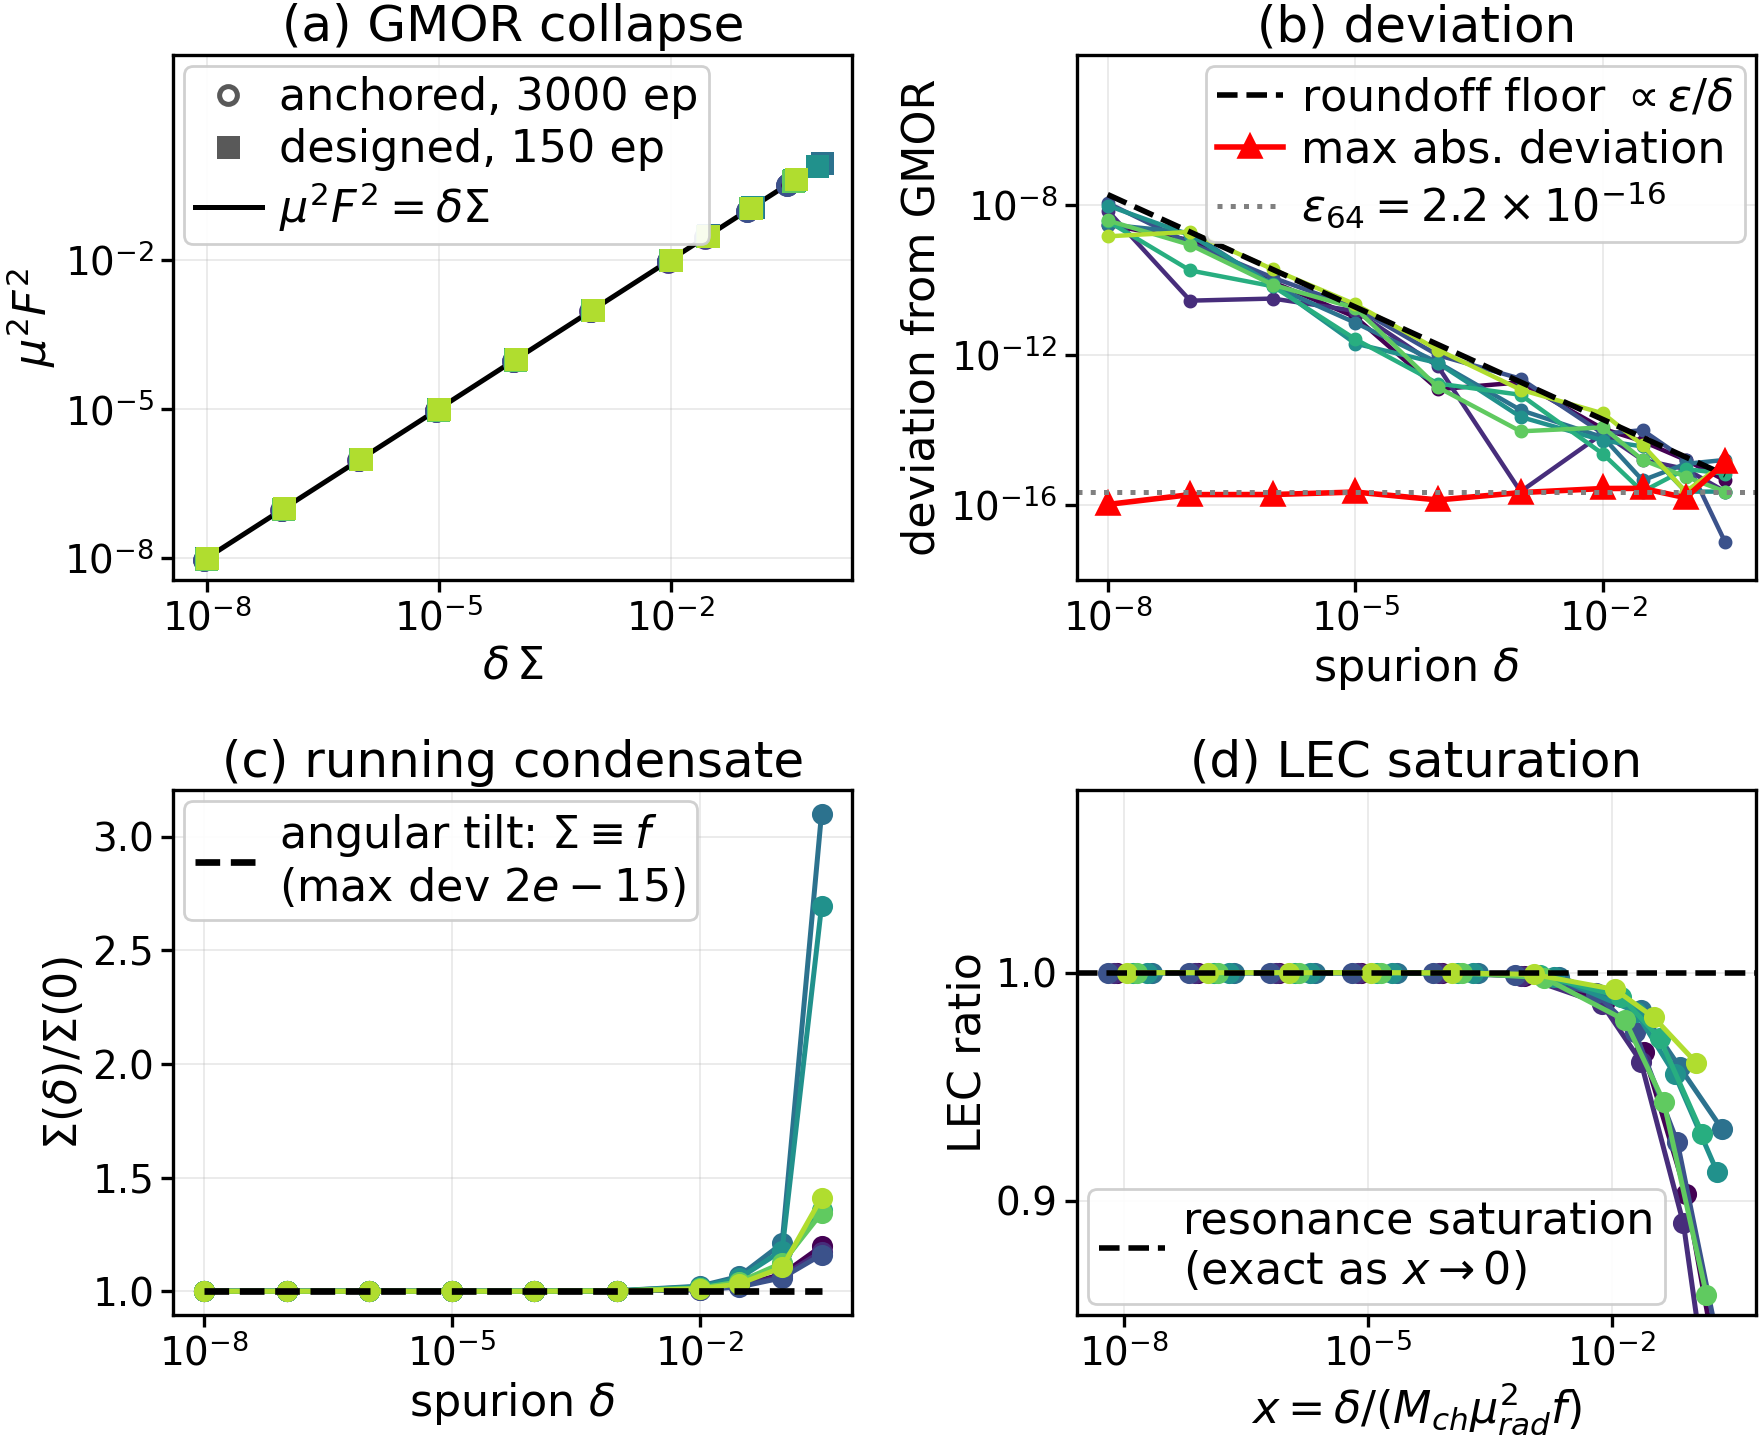
\includegraphics[width=\linewidth]{figs/fig3_gmor_condensate.png}
\caption{Full GMOR structural verification measured via a linear ambient spurion. (a) Total collapse of $\mu^2F^2=\delta\Sigma$ mapped precisely across $8$ decades of $\delta$ tracking. (b) Bound absolute deviations pinned at the exact $f64$ limits ($\le1.33{\times}10^{-15}$) juxtaposed against autodiff relative-roundoff thresholds. (c) The functional running condensate $\Sigma(\delta)/\Sigma(0)$ scaled against an angular tilt baseline. (d) The asymptotic alignment of the low-energy-constant ratio as the chiral expansion variable $x$ scales toward zero.}
\label{fig:gmor}
\end{figure}

\emph{\textbf{Precision fine print, next to the claim.}} GMOR holds to machine precision \textbf{in absolute terms at every $\delta$}; relative exactness ($\le2.7{\times}10^{-14}$) is demonstrated for $\delta\ge10^{-2}$. The growing \emph{relative} deviation at small $\delta$ is \textbf{not} a failure of the law but the roundoff floor of the \textbf{autodiff Hessian}: the angular curvature is $K_{\theta\theta}=\delta/r^*$, reconstructed as a difference of $O(\lVert K\rVert)$ terms, so its absolute error is $\sim\epsilon\lVert K\rVert$ and its relative error $\sim\epsilon/\delta$. This was confirmed directly: on the analytic Mexican hat a \textbf{cancellation-free} Hessian returns relative deviation $1.1$--$2.2{\times}10^{-16}$ at \emph{every} $\delta\in[10^{-8},0.3]$, while the autodiff Hessian on the same potential returns $2.28{\times}10^{-8}\to4.22{\times}10^{-15}$ across that range, exactly $\propto1/\delta$. \textbf{Do not quote ``$2.2{\times}10^{-16}$ relative'' for this experiment.} The same $\epsilon/\delta$ floor applies to every $\mu^2$ probe in this paper; all other sweeps here use $\delta\ge10^{-4}$, where the floor is $\sim10^{-12}$ and the quoted relative agreements are sound.

\textbf{G.5 The expansion variable, and where it stops being small.} With $\mu^2_{\rm LO}\equiv\delta\Sigma(0)/F^2(0)$, the theory predicts a \emph{relative} leading-order error $x\equiv\delta/(M_{\rm ch}\mu_{\rm rad}^2f)$; this is the $x$ of Figure~\ref{fig:gmor}(d). \textbf{Breakdown is visible and expected:} at $\delta=0.3$ the softest-radial seed, $\mu_{\rm rad}^2=0.670$, has $x=0.68$---not small---and $\Sigma$ has run $+210\%$, so the expansion is uncontrolled there and \textbf{$\delta=0.3$ must not be quoted for the next-to-leading-order claim}: cap at $x<0.25$ or state $x$ explicitly.

\textbf{G.6 Honest scope.} This appendix is tree-level and classical: no loops, chiral logarithms, running low-energy constants or anomalies. It is probe-only on already-trained checkpoints, with the spurion off by default so as to be bit-compatible with every result elsewhere, on one architecture family---designed exact $SO(2)$, dimension $4$, laptop CPU. The emergent MLP arm is untested and would carry its own self-breaking $\delta_{\rm eff}$, so GMOR there should be tested as $\delta\to\delta+\delta_{\rm eff}$: an open falsifiable, not a result.

\end{document}
